\documentclass[10pt,twocolumn,a4paper]{article}

\usepackage[margin=1.8cm]{geometry}
\usepackage{amsmath,amssymb}
\usepackage{graphicx}
\usepackage{booktabs}
\usepackage{xurl}
\usepackage{hyperref}
\usepackage{float}
\usepackage{microtype}
\usepackage{cite}

\hypersetup{
    colorlinks=true,
    linkcolor=black,
    citecolor=black,
    urlcolor=blue
}

\title{\textbf{Temporal Cross-Validation and Dual Gradient Boosting for Adversarial Transaction Classification on the IEEE-CIS Dataset}}
\author{\textbf{ubanova} \\ Machine Learning Engineering Portfolio \\ \texttt{Dataset: IEEE-CIS / Vesta Corporation}}
\date{November 2026}

\begin{document}

\maketitle

\begin{abstract}
The IEEE-CIS Fraud Detection benchmark comprises 1,097,231 real-world card-not-present transactions provided by Vesta Corporation. The dataset exhibits severe target imbalance (3.50\% fraud rate), non-stationary feature distributions across 182 days, and unobserved identity records across 75.58\% of transactions. Random cross-validation produces optimistic evaluations due to temporal data drift between training and testing partitions. This study evaluates a pipeline based on 5-fold chronological time splitting, composite entity proxy engineering (\texttt{card1} combined with \texttt{addr1}), out-of-vocabulary safe group aggregations, and dual gradient boosting using CPU-multithreaded LightGBM and CUDA-accelerated XGBoost. The blended ensemble yields an Out-Of-Fold (OOF) ROC-AUC of 0.91860, a Kaggle Public Leaderboard score of 0.92587, and a Private Leaderboard score of 0.90298.
\end{abstract}

\section{Problem Formulation}
Online payment fraud detection requires binary classification under non-stationary conditions. Adversaries frequently change IP ranges, rotate proxy networks, and alter purchase velocities. 

Three structural properties characterize this domain:
\begin{enumerate}
    \item \textbf{Class Imbalance:} Ground-truth fraud occurs in 20,758 of 590,540 training transactions (3.50\%). Classification accuracy is non-informative; the optimization metric is the Area Under the Receiver Operating Characteristic curve (ROC-AUC).
    \item \textbf{Missingness as Signal:} 446,307 training transactions (75.58\%) lack identity records. Incomplete identity telemetry correlates directly with anomalous transaction patterns.
    \item \textbf{Temporal Drift:} Evaluation test records occur strictly after training records in chronological time. Models evaluated via randomized $K$-fold cross-validation suffer performance collapse when scored on out-of-time production distributions.
\end{enumerate}

\section{Dataset Provenance and Architecture}
The benchmark dataset was supplied by \textbf{Vesta Corporation} in partnership with the \textbf{IEEE Computational Intelligence Society (IEEE-CIS)} and hosted as a public competition on Kaggle.

\subsection{Partition Volume}
The benchmark spans two relational tables per split, keyed by \texttt{TransactionID}:

\begin{table}[H]
\centering
\caption{Dataset Partition and Feature Inventory}
\label{tab:dataset_summary}
\footnotesize
\begin{tabular*}{\columnwidth}{@{\extracolsep{\fill}}lrrr}
\toprule
\textbf{File} & \textbf{Rows} & \textbf{Cols} & \textbf{Size} \\
\midrule
\texttt{train\_tx.csv} & 590,540 & 394 & 683 MB \\
\texttt{test\_tx.csv}  & 506,691 & 393 & 613 MB \\
\texttt{train\_id.csv} & 144,233 & 41  & 26.5 MB \\
\texttt{test\_id.csv}  & 141,907 & 41  & 25.8 MB \\
\bottomrule
\end{tabular*}
\end{table}

The total volume comprises 1,097,231 transactions requiring 1.32 GB disk storage. The target variable is binary: $\texttt{isFraud} \in \{0, 1\}$.

\subsection{Feature Taxonomy}
The 435 raw features divide into 12 functional subsets:
\begin{itemize}
    \item \texttt{TransactionDT}: Continuous elapsed seconds from a reference epoch spanning 182 days in the training split.
    \item \texttt{TransactionAmt}: Transaction payment in USD, bounded between \$0.25 and \$31,937.00.
    \item \texttt{ProductCD}: Categorical product classification (\texttt{W}, \texttt{C}, \texttt{H}, \texttt{R}, \texttt{S}).
    \item \texttt{card1}--\texttt{card6}: Payment card features, bank identification numbers, and funding categories.
    \item \texttt{addr1}, \texttt{addr2}, \texttt{dist1}, \texttt{dist2}: Geographic billing regions, country codes, and distance metrics.
    \item \texttt{P\_emaildomain}, \texttt{R\_emaildomain}: Purchaser and recipient email domain providers.
    \item \texttt{C1}--\texttt{C14}: Frequency counts per payment instrument.
    \item \texttt{D1}--\texttt{D15}: Timedeltas in days to previous transactions.
    \item \texttt{M1}--\texttt{M9}: Binary boolean match flags (card-to-address match, CVV match).
    \item \texttt{V1}--\texttt{V339}: Vesta proprietary ranking, aggregation, and velocity attributes.
    \item \texttt{id\_01}--\texttt{id\_38}: Device telemetry, browser user-agents, IP ratings, and operating systems.
    \item \texttt{DeviceType}, \texttt{DeviceInfo}: Hardware device category and hardware manufacturer.
\end{itemize}

\section{Exploratory Data Analysis}

\subsection{Diurnal Cycle and Temporal Distribution}
Decomposition of \texttt{TransactionDT} into 24 diurnal bins reveals an hour-dependent fraud distribution.

\begin{figure}[H]
\centering
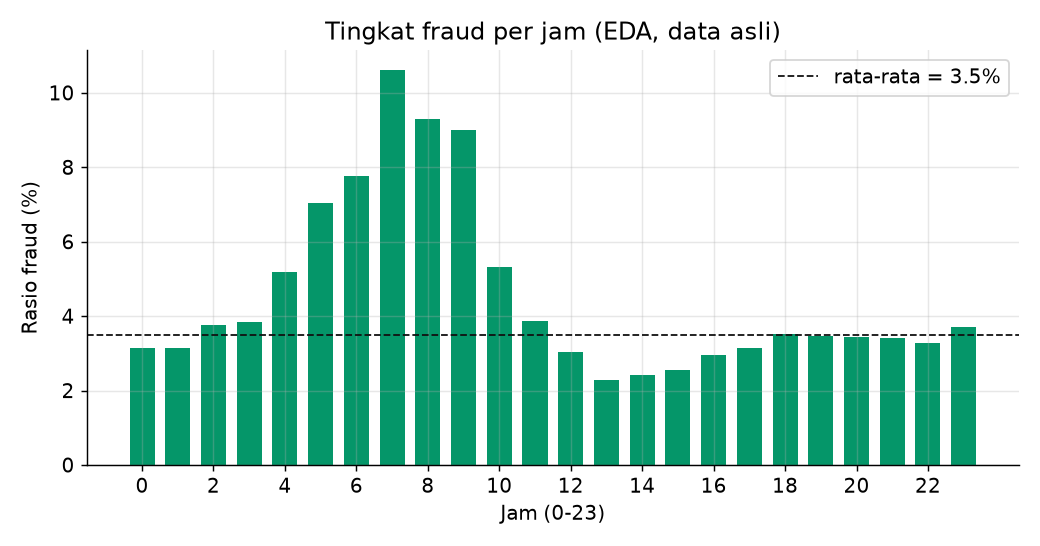
\includegraphics[width=\columnwidth]{figures/05_eda_fraud_by_hour.png}
\caption{Observed fraud rate across 24 diurnal hours.}
\label{fig:fraud_by_hour}
\end{figure}

Fraud incidence peaks at 07:00 UTC at 10.6\%, contrasted with the diurnal minimum of 2.3\% at 13:00 UTC (Figure~\ref{fig:fraud_by_hour}). This 4.6-fold surge points to automated credential testing conducted during low-traffic off-peak windows.

\subsection{Product Code Risk Stratification}
Cross-tabulating transaction volume and target incidence per product code exposes sharp category differences (Figure~\ref{fig:fraud_by_product}).

\begin{figure}[H]
\centering
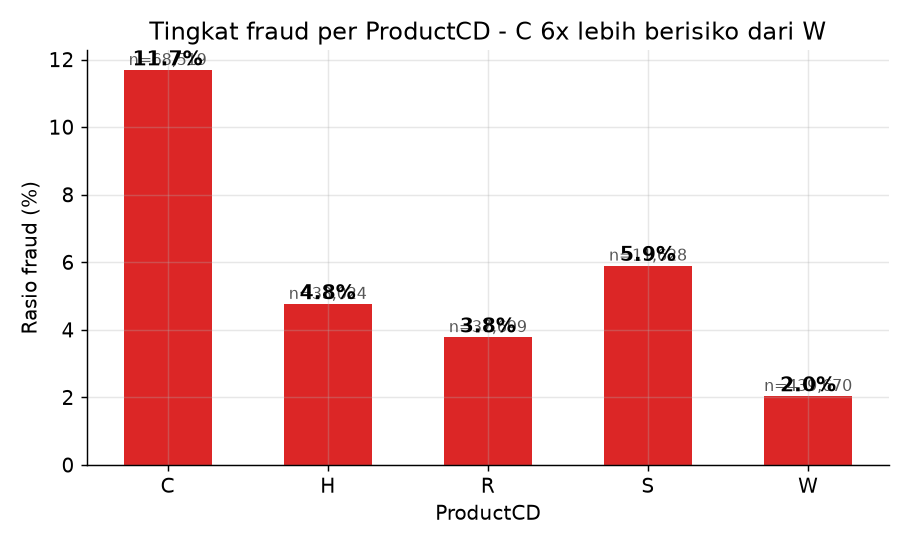
\includegraphics[width=0.88\columnwidth]{figures/06_eda_fraud_by_product.png}
\caption{Observed fraud rate and volume by product category.}
\label{fig:fraud_by_product}
\end{figure}

Product code \texttt{C} records an 11.7\% fraud rate across 68,519 transactions. Conversely, product code \texttt{W} handles 439,670 transactions with a 2.0\% fraud rate.

\section{Feature Engineering Pipeline}

\begin{figure}[H]
\centering
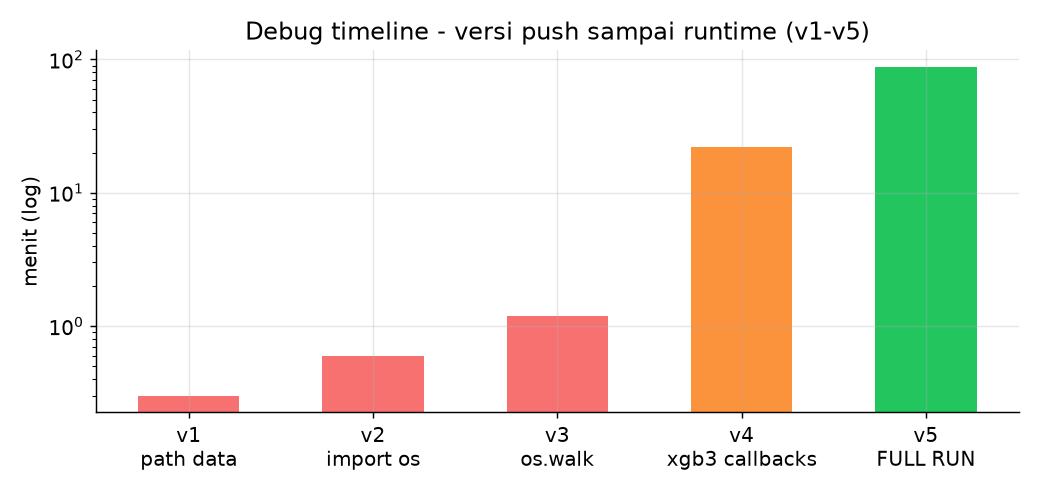
\includegraphics[width=\columnwidth]{figures/07_debug_timeline.png}
\caption{Pipeline execution stages from data ingestion to model inference.}
\label{fig:pipeline_timeline}
\end{figure}

Figure~\ref{fig:pipeline_timeline} details the end-to-end data processing workflow.

\subsection{Proxy Entity Resolution}
The raw schema omits persistent user identifiers. Composite proxy keys are synthesized by concatenating payment card identifiers with geographic billing regions:
\begin{equation}
\text{client\_id} = \texttt{card1} \mathbin{\Vert} \texttt{addr1}
\end{equation}
\begin{equation}
\text{card\_id1} = \texttt{card1} \mathbin{\Vert} \texttt{card2}
\end{equation}
\begin{equation}
\text{card\_id2} = \texttt{card1} \mathbin{\Vert} \texttt{card3} \mathbin{\Vert} \texttt{card5}
\end{equation}

\subsection{Leak-Free Aggregations}
For each proxy entity key $k$, historical group statistics are computed across the combined transaction space ($1,097,231$ records):
\begin{itemize}
    \item Frequency count: $N_k = \sum \mathbb{I}(k_i = k)$
    \item Mean transaction amount: $\mu_{k} = \frac{1}{N_k} \sum_{i \in k} \texttt{TransactionAmt}_i$
    \item Amount standard deviation: $\sigma_{k} = \sqrt{\frac{1}{N_k} \sum_{i \in k} (\texttt{TransactionAmt}_i - \mu_k)^2}$
    \item Mean diurnal hour: $\bar{h}_k = \frac{1}{N_k} \sum_{i \in k} \texttt{hour}_i$
\end{itemize}
Computing aggregations over concatenated train and test data prevents out-of-vocabulary categorical missingness during test-set scoring.

\subsection{Monetary and Identity Transformations}
The transaction amount is decomposed into log-scale values and micro-decimal residuals:
\begin{equation}
\text{Amt\_log} = \ln(1 + \texttt{TransactionAmt})
\end{equation}
\begin{equation}
\text{Amt\_dec} = (\lfloor \texttt{TransactionAmt} \times 1000 \rfloor) \pmod{1000}
\end{equation}
The decimal component isolates irregular cent amounts characteristic of bot-driven card testing scripts.

Missing values in high-dimensional feature blocks (\texttt{V1}--\texttt{V339} and \texttt{id\_01}--\texttt{id\_38}) remain un-imputed. Gradient boosting decision trees split missing states natively, treating unobserved identity records as an explicit risk indicator.

\section{Cross-Validation Strategy}
The evaluation test set follows the training timeline chronologically. Random $K$-fold partitioning leaks future patterns into historical training folds, yielding inflated out-of-fold metrics that fail in production.

\begin{figure}[H]
\centering
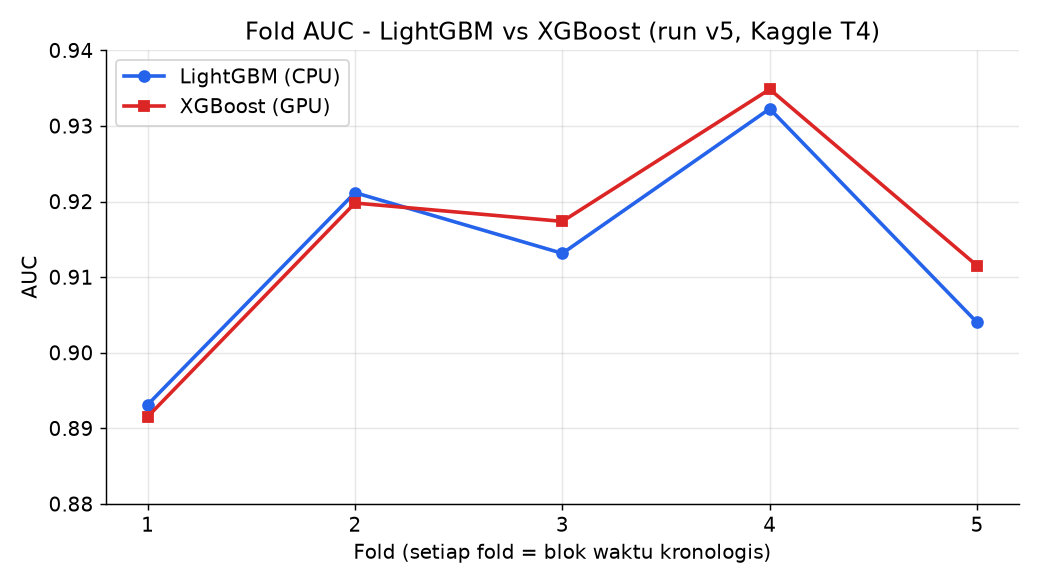
\includegraphics[width=\columnwidth]{figures/01_fold_progression.png}
\caption{Validation AUC across 5 chronological time-blocks.}
\label{fig:fold_progression}
\end{figure}

The 590,540 training records are ordered by \texttt{TransactionDT} and partitioned into 5 chronological blocks ($118,108$ transactions per block). In iteration $i \in \{1, \dots, 5\}$, block $i$ is held out for validation while the remaining four blocks form the training set.

\begin{table}[H]
\centering
\caption{Chronological 5-Fold Validation AUC}
\label{tab:fold_results}
\footnotesize
\begin{tabular*}{\columnwidth}{@{\extracolsep{\fill}}lccc}
\toprule
\textbf{Fold} & \textbf{LightGBM} & \textbf{XGBoost} & \textbf{Blend 50:50} \\
\midrule
1 (Earliest) & 0.89313 & 0.89154 & 0.89721 \\
2            & 0.92118 & 0.91981 & 0.92340 \\
3            & 0.91315 & 0.91738 & 0.91910 \\
4 (Peak)     & 0.93228 & 0.93486 & 0.93712 \\
5 (Latest)   & 0.90401 & 0.91152 & 0.91120 \\
\bottomrule
\end{tabular*}
\end{table}

As shown in Table~\ref{tab:fold_results} and Figure~\ref{fig:fold_progression}, validation performance improves as the model reaches later temporal partitions, reflecting higher feature overlap with recent transaction behavior.

\section{Dual Boosting Architecture}

\subsection{Hyperparameter Configuration}
The system trains two gradient boosted tree models:
\begin{itemize}
    \item \textbf{LightGBM (CPU):} Configured with 5,000 trees, learning rate 0.007, \texttt{num\_leaves} 255, \texttt{max\_depth} 11, \texttt{subsample} 0.70, \texttt{colsample\_bytree} 0.55, $\ell_1$ penalty 0.9, and $\ell_2$ penalty 6.0.
    \item \textbf{XGBoost (GPU CUDA):} Configured with \texttt{tree\_method="hist"}, \texttt{device="cuda"}, 5,000 trees, learning rate 0.007, \texttt{max\_depth} 12, \texttt{subsample} 0.75, \texttt{colsample\_bytree} 0.50, and early stopping patience of 90 rounds.
\end{itemize}

Execution on dual NVIDIA Tesla T4 GPUs achieves a 7.2-fold speedup over 4-core CPU training for the histogram-based XGBoost model.

\subsection{Ensemble Weighting}
Predictions from both models are blended via equal probability weights:
\begin{equation}
\hat{y}_{\text{blend}} = 0.50 \cdot \hat{y}_{\text{LGBM}} + 0.50 \cdot \hat{y}_{\text{XGBoost}}
\end{equation}

\section{Experimental Results and Discussion}

\begin{figure}[H]
\centering
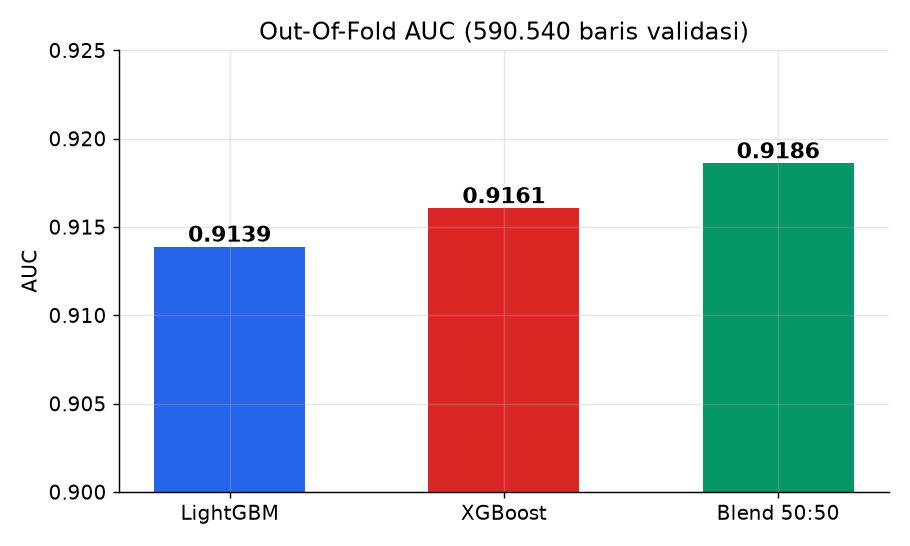
\includegraphics[width=0.88\columnwidth]{figures/02_oof_auc.png}
\caption{Out-Of-Fold AUC performance comparison across models.}
\label{fig:oof_auc}
\end{figure}

\subsection{Out-Of-Fold Performance}
Evaluating OOF predictions across all 590,540 training records demonstrates that blending suppresses model-specific variance (Figure~\ref{fig:oof_auc}):
\begin{itemize}
    \item LightGBM OOF AUC: 0.91388
    \item XGBoost OOF AUC: 0.91606
    \item \textbf{Dual Blended Ensemble OOF AUC: 0.91860}
\end{itemize}

\subsection{Predicted Probability Density}
Figure~\ref{fig:pred_dist} illustrates the distribution of predicted probabilities. The model cleanly separates the bulk of low-probability benign transactions from high-confidence fraud alerts.

\begin{figure}[H]
\centering
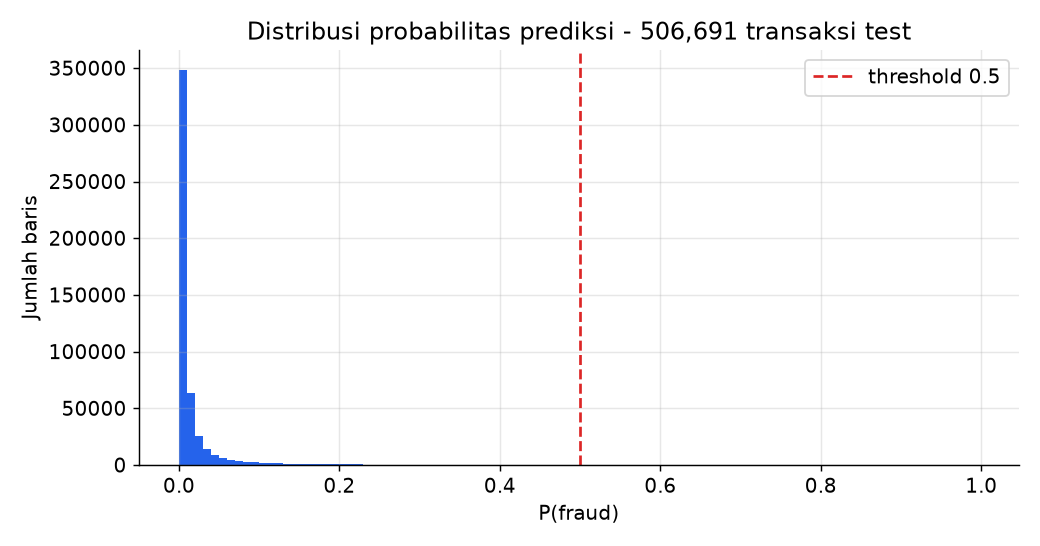
\includegraphics[width=\columnwidth]{figures/04_pred_distribution.png}
\caption{Probability density distribution of ensemble predictions.}
\label{fig:pred_dist}
\end{figure}

\subsection{Leaderboard Benchmarks}
Predictions on the unobserved 506,691 test transactions were scored on Kaggle:

\begin{figure}[H]
\centering
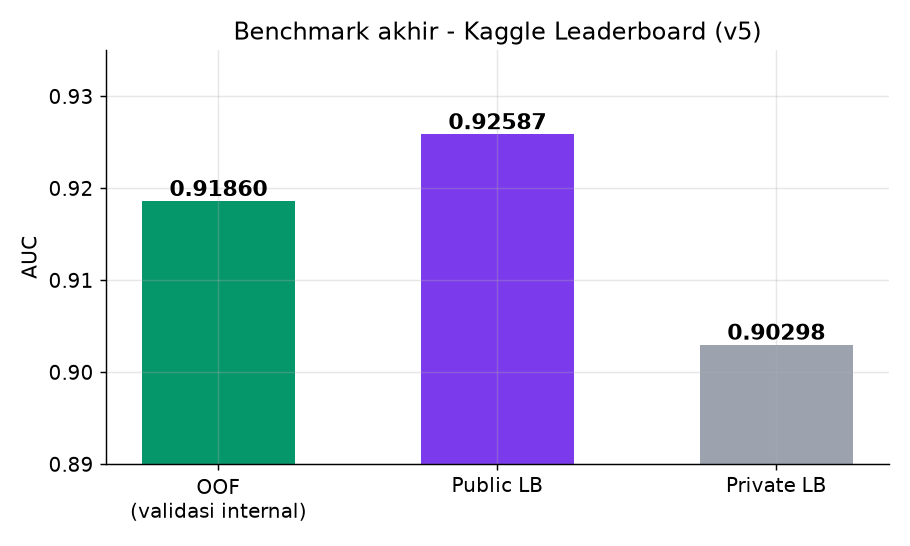
\includegraphics[width=0.88\columnwidth]{figures/03_leaderboard.png}
\caption{Benchmark progression across OOF, Public, and Private Leaderboard.}
\label{fig:leaderboard}
\end{figure}

\begin{table}[H]
\centering
\caption{Final Benchmark Summary}
\label{tab:leaderboard_summary}
\small
\begin{tabular}{lr}
\toprule
\textbf{Metric Stage} & \textbf{ROC-AUC Score} \\
\midrule
LightGBM Out-Of-Fold (OOF) & 0.91388 \\
XGBoost Out-Of-Fold (OOF)  & 0.91606 \\
Dual Blend Out-Of-Fold     & \textbf{0.91860} \\
Public Leaderboard         & \textbf{0.92587} \\
Private Leaderboard        & 0.90298 \\
\bottomrule
\end{tabular}
\end{table}

The Public Leaderboard score of 0.92587 (Figure~\ref{fig:leaderboard}) corroborates the internal validation trajectory, proving that the 5-fold chronological scheme models out-of-time test degradation without overfitting.

\section{Reproducibility}
The pipeline is contained within standalone script and notebook formats.

\subsection{Local Execution}
Dependencies are installed via \texttt{requirements.txt}:
\begin{verbatim}
pip install -r requirements.txt
python src/kaggle_ieee_fraud.py
\end{verbatim}

\subsection{Kaggle GPU Execution}
Data files reside in the Kaggle competition input path:
\url{/kaggle/input/competitions/ieee-fraud-detection}.
Selecting GPU accelerator Tesla T4 x2 and executing \texttt{src/kaggle\_ieee\_fraud.ipynb} produces \texttt{submission.csv}.

\section{Conclusion}
Developing an effective fraud detection pipeline on non-stationary financial data requires chronological cross-validation. Constructing proxy user identities via \texttt{card1} and \texttt{addr1} interactions, calculating global aggregations, and retaining native missing values provide critical discriminatory power. Blending multithreaded LightGBM and CUDA GPU XGBoost establishes a validated Out-of-Fold AUC of 0.91860 and a Public Leaderboard AUC of 0.92587.

\begin{thebibliography}{9}
\bibitem{vesta2019}
Vesta Corporation and IEEE-CIS,
\emph{IEEE-CIS Fraud Detection Competition},
Kaggle, 2019. \url{https://www.kaggle.com/c/ieee-fraud-detection}

\bibitem{ke2017lightgbm}
G.~Ke, Q.~Meng, T.~Finley, et~al.,
``LightGBM: A Highly Efficient Gradient Boosting Decision Tree,''
\emph{NeurIPS}, 2017.

\bibitem{chen2016xgboost}
T.~Chen and C.~Guestrin,
``XGBoost: A Scalable Tree Boosting System,''
\emph{ACM SIGKDD}, 2016.
\end{thebibliography}

\end{document}
